\documentclass[11pt]{article}
\usepackage[margin=1in]{geometry}
\usepackage{enumerate}
\usepackage{framed}
\usepackage{multirow}
\usepackage{multicol}
\usepackage{bm}
\usepackage{amssymb}
\usepackage{amsmath}
\usepackage{amsthm}
\usepackage{multicol}
\usepackage{graphicx}
\usepackage{float}
\setlength{\columnsep}{1in}
\begin{document}

\newcommand{\Name}[1]{\noindent \textbf{Name:} #1 \\}
\newcommand{\pderiv}[2]{\frac{\partial #1}{\partial #2}}
\newcommand{\psderiv}[3]{\frac{\partial^2 #1}{\partial #2 \partial #3}}

\begin{center}
	\bf
	Machine Learning \\
	Computer Science 158 \\
	Spring 2017 \\
	\rm
	Project 7\\
\end{center}
\noindent \textbf{Name: Varsha Kishore and Savannah Baron} \\

\begin{enumerate}[1]
\item PCA and Image Reconstruction
\begin{enumerate}[(a)]
\item The average face seems to face on common features like eyes, nose and mouth that are in every picture in the data set. 
\item In the first 12 principle components, we can see different images representing different aspects of faces that might offer the most variance. For instance, in the first three, there is a lot of emphasis on color and face shape, where as the 8th we see features, and in the last two we see what seem to be faces ordered in different directions.  The principle components seek to explain the highest variance dimensions of the data. Thus, by emphasizing features such as face shape, eyes/mouth/nose and face angle, the principle components here represent important elements of faces.
\item Some people seem to be represented more clearly with lower $l$'s. For some of the other faces we need $l$ to be $100$ or higher for the face to become clear. 
\end{enumerate}
\item $K$-Means and $K$-Medoids
\begin{enumerate}[(a)]
\item This is a bad idea because the quantity $J$ will be minimized when the number of clusters
is $n$, and each cluster centroid corresponds to a data point in the training set. In other words, if we
also minimize with respect to $k$, we will massively overfit the data. 
\item Code complete!
\item Code complete!
\item Code complete!
\item Code complete!
\end{enumerate}
\item Clustering Faces
\begin{enumerate}[(a)]
\item \begin{tabular}{| c | c | c | c |}
  \hline		
   & Average & Min & Max \\
  \hline
  k-means & 0.616875 & 0.55 & 0.775 \\
  k-medoids & 0.63125 & 0.575 & 0.725   \\
  \hline
\end{tabular}\\ \\
K-means took around $1$ second to run and k-medoids took around $3$ seconds to run. Looking at the numbers in the table above, it seems like k-medoids very slightly outperformed k-means. k-medoids seems to have a smaller variance. 
\item In this graph we see that k-medoids outperforms k-means for every $l$ except for $l=1$. We also see that the performance initially increases or stays constant as $l$ increases (roughly until $l=10$), then the performance decreases. We need enough principle components to represent the variance in the images, so for the first few values of $l$, performance increases. When $l$ become greater than $20$ there might be issues due to higher dimensionality and noise that leads to reduced scores.  \\
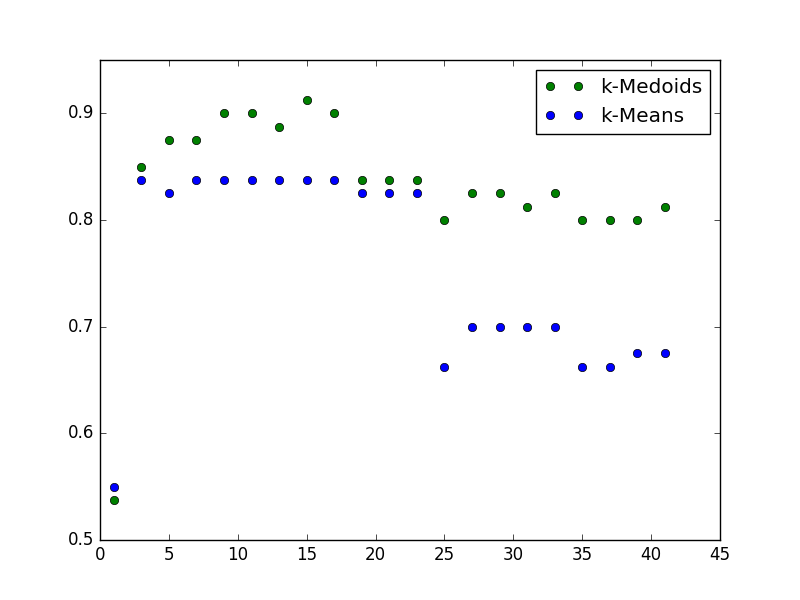
\includegraphics[scale=0.7]{figure_1}
\item We first wanted to identify two faces that are similar and two faces that are dissimilar. We did this by computing "average face" (average of all the features) for every person. Then we found two people who had averages face values that were very close (the classes corresponding to these people are $0$ and $2$) and two people who had averages face values that were far apart (the classes corresponding to these people are $13$ and $16$). From previous parts, we saw that k-medoids performed slightly better. So, we used k-medoids to see how well the algorithm performs when we try to cluster classes $0,2$ and when we try to cluster classes $13,16$. We found that the average score for $0,2$ was $0.5275$ and the average score for $13, 16$ was $0.9325$. As expected the classifier was able to perform better when it was clustering two dissimilar faces.  The table below shows the results that we got: \\
 \begin{tabular}{| c | c | c | c |}
  \hline		
   & Average & Min & Max \\
  \hline
  Classes $0$ and $2$ & 0.5275 & 0.5 & 0.55 \\
  Classes $13$ and $15$ & 0.9325 & 0.925 & 0.9375   \\
  \hline
\end{tabular}\\ \\
\end{enumerate}
\item Extra Credit! \\
To initialize $k$ centers we decided to use the following approach. We first pick one random point $p$ from the given $n$ points. Then we compute the distance from $p$ to each of the other points. We sort the distances we computed in ascending order. We pick $k$ evenly separated values from the sorted distances list and find the points corresponding to these distance values and assign those points as centers. We think this is a better way of initializing centers because we are ensuring that the centers are spread apart the entire space. \\
Our initialization scheme does perform better. Here's a table looking at values we got when we used randomInit, cheatInit and our own init scheme. \\
 \begin{tabular}{| c | c | c | c |}
  \hline		
   & Average & Min & Max \\
  \hline
  K-means: random & 0.5275 & 0.5 & 0.55 \\
  K-medoids: random $13$ and $15$ & 0.9325 & 0.925 & 0.9375   \\
K-means: cheat & 0.5275 & 0.5 & 0.55 \\
  K-medoids: cheat $13$ and $15$ & 0.9325 & 0.925 & 0.9375   \\
K-means: our init & 0.5275 & 0.5 & 0.55 \\
  K-medoids: our init $13$ and $15$ & 0.9325 & 0.925 & 0.9375   \\
  \hline
\end{tabular}

 \end{enumerate}


\end{document}
